\section{Validation}

This section reviews the validation of immersed boundary methods.
The main goal of the validation is to determine the numerical error and the
numerical stability of an immersed boundary method.
Furthermore it is important to test if conservation laws, in particular the conservation of mass,
are fulfilled.

In the first part of the chapter an introduction to different test cases
will be given. Three different test problems were chosen.
The flow between to planes, also known as Planar Poiseuille flow, the flow in a Pipe, referred to as Hagen-Poiseuille flow and the flow
between two rotating cylinders, know as the Taylor-Couette system.
In the second part of the chapter the result for the different test cases will be presented and discussed.

\paragraph{Conventions}\mbox{}\\

In this section the following abbreviations will be used

\begin{multicols}{2}
\begin{description}
    \item[VP]{Volume-Penalization Method}
    \item[DF]{Direct Forcing Method}
    \item[IP]{Interpolation Method}
    \item[VF]{Volume-Fraction Extension}
    \item[o2]{Finite Difference Schemes of 2nd order}
    \item[o4]{Finite Difference Schemes of 4th order}
\end{description}
\end{multicols}

For example, DF-VF-o2 method, refers to the Direct-Forcing method, extended with the Volume-Fraction
method and the use of 2nd order Finite Difference Schemes.

%In general it is necessary to obtain a good evaluation of the numerical truncation error,
% the numerical stability over longer periods of time
%and Grid convergence studys against theoretical and high-resolution numerical solutions
%will be performed and compared for the different IBMs.
%This part of the thesis the thesis deals with the numerical validation of the immersed
%boundary methods
%In order to ensure a correct numerical behavior of the introduced methods, a
%Multiple examples from simple to more complex test cases are introduced in this section.
\clearpage

\subsection{Laminar Poiseuille-Flow}

\begin{figure}[!bp]
  \begin{minipage}[c]{0.6\textwidth}
      \centering
        \resizebox{0.9 \textwidth}{!}{
       \import{gfx/immersed_boundary/poiseuille_flow//}{setup.pdf_tex}
      }
  \end{minipage}
  \begin{minipage}[c]{0.3\textwidth}
      \caption{Setup of the Poiseuille-flow channel.
      \label{validation:setup_pf}
      }
  \end{minipage}
\end{figure}

The first test case is the laminar poiseuille-flow. The theoretical setup is presented in Fig. \ref{validation:setup_pf}.
It consist of two infinite extending  planes at $z=h_1$ and $z=h_2$, which are oriented
parallel to the xy-plane, at a distance $\Delta h = h_2 - h_1$.
Numerically this is realized by using periodic boundaries in xy-direction and
No-Slip boundaries in the z-direction.

The velocity profile is a result from a predefined spatial constant pressure gradient $\nicefrac{\partial p}{\partial x}$
 in x-direction, that is added into the Navier-Stokes equation.
The steady state for the non-dimensional equations is given by \citep{}
\begin{align}
    \label{vali:pflow_navstok}
    \frac{\partial v_x}{\partial t} &= - \frac{\partial p}{\partial x}
     + \frac{1}{Re} \frac{\partial^2 v_x}{\partial z^2} = 0
\end{align}

with the Reynolds-number defined as $Re = \nicefrac{V_{m}\Delta h}{\nu}$.
For this system the non-dimenzionalization is given by the scales
    $r^* = \nicefrac{r}{\Delta h}$, $v^*=\nicefrac{V_(\text{m})}{\Delta h}$,
    $t^* = \nicefrac{V_{\text{m}}}{\Delta h}$ and $p^* = p \rho V_{\text{max}}^2$.

\clearpage
The velocity $V_m$ is defined as $\max(v_x(z))$.
An integration of Eq. \ref{vali:pflow_navstok} gives
\begin{align}
v_z &= \frac{1}{2}\frac{\partial p}{\partial x}z^2 + zc_1 + c_2
\end{align}

Using the NoSlip-boundary condition $v_x(h_1) = v_x(h_2) = 0$ and furthermore by defining
$A:=\frac{1}{2}\frac{\partial p}{\partial x} Re$ one obtains the additional conditions

\begin{align}
c_1 &= A\frac{h_1^2 -h_2^2}{h_2 - h_1} = -A(h_1+h_2)\\
c_2 &= A(h_1(h_1 + h_2) - h_1^2) = Ah_1h_2\\
\end{align}

The velocity is than given by the quadratic function

\begin{align}
\label{vali:pflow_theosol}
v_x &= A(z^2 - z(h_1 + h_2) + h_1h_2)
\end{align}

The maximum velocity and position are given by
\begin{align}
z_{max} &= \frac{h_1+h_2}{2} \wedge v_{max} = A\left(h_1h_2 - \frac{(h_1 + h_2)^2}{4}\right)
\end{align}

$V_{m}$ has to be 1 by the definition of the non-dimensionalzation. This gives
\begin{align}
\frac{\partial p}{\partial x} &= \frac{2}{Re}\frac{1}{\left(h_1h_2 - \frac{(h_1+h_2)^2}{4} \right)}
\end{align}
as a necessary condition for the pressure gradient.\\
\clearpage

\subsection{Simulations}

The Poiseuille-flow test case is used in particular as a first validation
for the Volume-Penalization and Direct-Forcing methods.

\subsubsection{Test of the Default Setup}

The purpose of the first simulation is the test of the default
implementation of the algorithm, without the use of immersed boundaries.
For this test case this is still possible since the geometry is non-curved
and parallel to the cartesian grid.
A grid convergence test was performed with the main simulation parameters given by

\begin{center}
\vspace*{0.7ex}
\begin{tabular}{c|c|c|c|c|c|c }
 $ N  $                   & $\Delta t$ & $\Delta x$            & $\Rey$  & $c^2$   & $l_x, l_y, l_z$ & $T_{end}$\\
\hline
 $[8, 256], \Delta N = 8 $& $10^{-4}$ & $\nicefrac{1}{N - 1}$ & 500     & $500$   & (1, 1, 1)       & 10\\
\end{tabular}
\vspace*{0.7ex}
\end{center}

The simulations were performed for finite difference schemes of 2nd and 4th order.

\subsubsection{Test of the Volume Penalization Method}

%With the given theoretical solution, the next objective is the comparison
%to the default implementation, the volume penalization method and the direct forcing method.
%Since we have a flow parallel to the grid  it does not make sence to compare it to the interpolation methods
%For the comparision with a theoretical solution it is necessary to ensure that
% the surface grid points match with the total height $h$ of the channel.

For the immersed boundary methdos the upper- and lower boundaries of the channel are realized by the masking function.
\begin{align}
H(x, y, z) = \begin{cases}
                    0, & \text{for \  }  h_1 \leq z \leq h_2 \\
                    1, & \text{else}.
             \end{cases}
\end{align}

For the volume penalization method we furthermore obtain a
The non-dimensionalized damping force  given by

\begin{align}
    \vec{f} = \frac{H}{J}v
\end{align}

where $J = \nicefrac{V_{m}}{\eta}$.

\clearpage

A first test is to investigate the error of the velocity profile, with a variation of the Reynolds-number and the damping rate $J$.
The total simulation domain is set to the height $l_z=2$ with $h_1=0.25$ and $h_2=0.75$.
A simulation series was performed with the main simulation parameters given by


\begin{center}
\vspace*{0.7ex}
\begin{tabular}{c|c|c|c|c|c|c|c }
 $ \Rey  $                      & $J$ &  $\Delta t$ & $\Delta x$            & $\Rey$  & $c^2$   & $l_x, l_y, l_z$ & $T_{end}$\\
\hline
 $[100, 500], \Delta \Rey = 25 $& $[10^{-5}, 5\cdot10^{-1}]  $ &  $10^{-4}$ & $\nicefrac{1}{N - 1}$ & 500     & $500$   & (1, 2, 0.25)  & 10\\
\end{tabular}
\vspace*{0.7ex}
\end{center}

The damping force was divided by 2 or 5 for n times(EXPLAIN).
To make sure that the channel width is equal to $\Delta h = 1$, the total height was set to $l_z\approx2.01587$.
This ensures that the grid points overlap exactly with the masking function at $h_1=0.25$ and $h_2=0.75$.
The simulations were performed for the 2nd order method. (O4 EXPLAIN)

As a second test a grid convergence study was carried out, with a constant Reynolds number and $J \in [1-23]$.
The resolution was varied between $N\in [4, 400]$ with $\Delta N = 4$, 2nd and 4th order schemes were tested.

\begin{center}
\vspace*{0.7ex}
\begin{tabular}{c|c|c|c|c|c|c|c }
 $ \Rey  $                      & $J$ &  $\Delta t$ & $\Delta x$            & $\Rey$  & $c^2$   & $l_x, l_y, l_z$ & $T_{end}$\\
\hline
 $[100, 500], \Delta \Rey = 25 $& $[10^{-5}, 5\cdot10^{-1}]  $ &  $10^{-4}$ & $\nicefrac{1}{N - 1}$ & 500     & $500$   & (1, 2, 0.25)  & 10\\
\end{tabular}
\vspace*{0.7ex}
\end{center}

\subsubsection{Test of the Direct Forcing Method}

Since the direct forcing method does not depend on a damping parameter it is sufficient enough
to carry out a grid convergence study
The simulation parameter are given by

\begin{center}
\vspace*{0.7ex}
\begin{tabular}{c|c|c|c|c|c|c|c }
 $ \Rey  $                      & $J$ &  $\Delta t$ & $\Delta x$            & $\Rey$  & $c^2$   & $l_x, l_y, l_z$ & $T_{end}$\\
\hline
 $[100, 500], \Delta \Rey = 25 $& $[10^{-5}, 5\cdot10^{-1}]  $ &  $10^{-4}$ & $\nicefrac{1}{N - 1}$ & 500     & $500$   & (1, 2, 0.25)  & 10\\
\end{tabular}
\vspace*{0.7ex}
\end{center}

2nd and 4th order finite difference schemes were tested.

\clearpage

\subsection{Results}
\subsubsection{Default seutp}

The results of the grid convergence study are shown in Fig. \ref{fig:ema1}.
The double logarithmic axis shows the dependency of the computed relative $l_2$-error norm
with respect to the grid resolution.

On this scale, the 4th order finite difference scheme has a linear decreasing error.
For the smallest resolution $N=8$ the error is of order $10^{-3}$,
in contrast to the highest resolution $N=256$ with an error of order $10^{-6}$
A convergence rate of the error  was computed by linear interpolation in the log-log space,
the results is about -2.257.
Hence, it can be said that the accuracy of the method is of 2nd order for this test case,
which is is in contradiction with the theory.

The error of the 2nd order finite difference scheme is of the order $10^{-8}$.
The value is approximately constant and not depend of the grid resolution.

\begin{figure}[!bp]
    \centering
    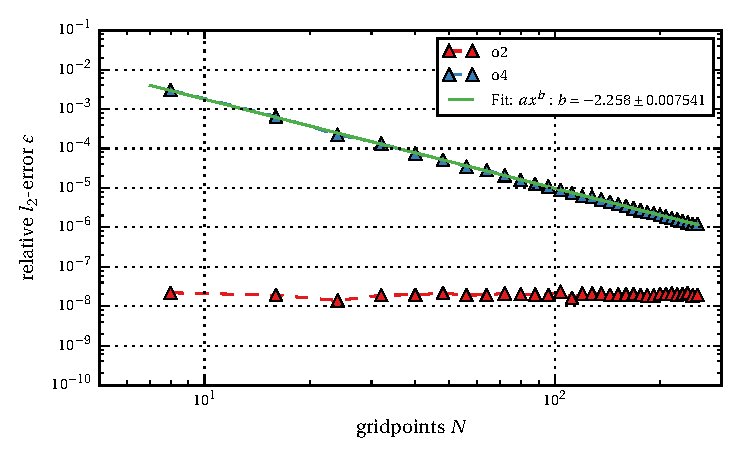
\includegraphics{gfx/immersed_boundary/poiseuille_flow/1_default/relative_l2error.pdf}
    \caption{Relative $l_2$-error for 2nd and 4th order finite difference schemes of the default algorithm without the use of an immersed boundary.\label{fig:ema1}}
\end{figure}

\clearpage


\subsubsection{Test of the Volume Penalization Method}

The first simulation was  a parameter study with variable Reynolds number $Re$ and damping rate $J$.
A first impression of the influence of the damping rate $J$ , is given by the velocity profiles of the numerical solution.
This is exemplarily shown in Fig. \ref{fig:vp_flow}, for variable $J$ and a constant reynolds number $Re=500$.
It can be noted that with an decrease of $J$, the numerical solution converges against the theoretical one.

\begin{figure}[!b]
  \centering
  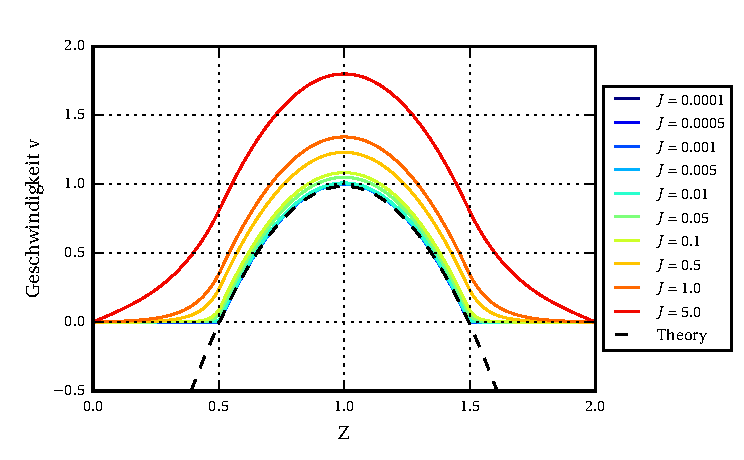
\includegraphics{gfx/immersed_boundary/poiseuille_flow/2_vp/vp_profile.pdf}  \caption{\label{fig:vp_flow}
    Velocity profile of the numerical solution with variable $J$ and $\Rey = 500$.}
\end{figure}

Furthermore it can be seen that the quadratic part of the velocity profile,
inside of the fluid domain ($0.5\leq z \leq 1.5$), is independent of the damping constant $J$.
Merely a slight offset at the boundaries creates a constant shift of the velocity profile.
In the masked area of the volume a decrease in velocity is visible which could  eventually be described by an
exponential law.

For an error estimation, the relative $l_2$-error was computed.
The results for the 2nd order scheme are shown in Fig. \ref{fig:vp_error}.
\begin{figure}[!b]
  \centering
  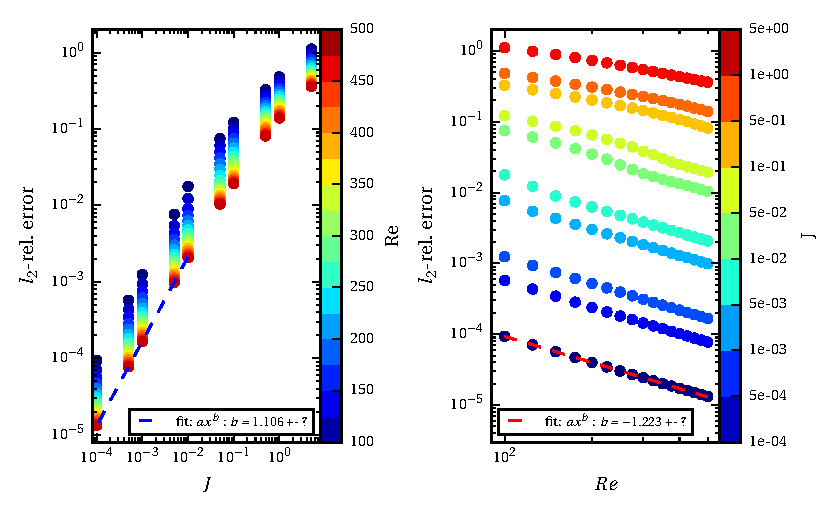
\includegraphics{gfx/immersed_boundary/poiseuille_flow/2_vp/vp_error.pdf}  \caption{\label{fig:vp_error}
    Relative $l_2$-error for variable damping rate $\nu$ and Reynolds number $Re$.}
  \centering
  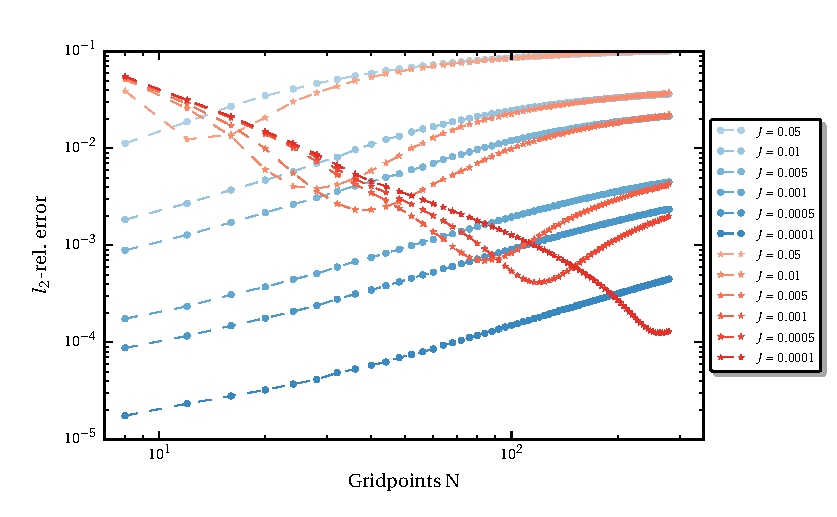
\includegraphics{gfx/immersed_boundary/poiseuille_flow/2_vp/vp_convergence.pdf}
  \caption{\label{fig:vp_conv}
      Relative $l_2$ error for variable damping rate $J$, for 2nd (blue) and 4th (red) order finite difference schemes.}
\end{figure}

On the left side of the plot the relative error is plotted against the damping rate, the reynolds number is
varied over a color scale. On the right side both variables are switched.

A decrease in the damping rate $J$ results in an decrease of the error about four orders, from $10^{-1}$ to $10^{-5}$.
With a change of the Reynolds number from $500$ down to $100$ the error decrease about one order.
It can be noticed that with an decrease of $\Rey$ or $J$ the error decreases linear in the log-log space.
For a small damping ($J>10^{-3}$) a breakdown of the linear relation can be observed.
This is an error resulting from the numerical setup.
\clearpage

The damping in the masking area is so weak that the flow reaches the  boundaries of the numerical domain.
This is not the case for $J<1e-3$ since the velocity profile is zero before it reaches the boundaries.\\
A linear fit in the log-log space gives a  decay rate of about $1.106$ for  $J$ and about $-1.223$ for $\Rey$.

The second part of the test was a grid convergence study with a constant Reynolds number, variable $J$ and grid resolution $N$.
The results are shown in Fig. \ref{fig:ema1}.

It can be noticed that a decrease in $\nu$ creates a shift in the error profile to overall smaller values.
However it is also noticable that the error of the 2nd order scheme, increases together with the resolution.
Even less understandable is the error function for the 4th order scheme.
With increasing resolution  a decrease into a minimum, followed by an increase can be observed.

The position of minimum is shifted to the right with an decrease of $J$.
For a constant $J>10^{-4}$ it is visible that the error for both methods converges against a
constant error  with an increase in the resolution.

\subsubsection{Direct Forcing Method}

The results of the grid convergence study are similat to the results of the default implementation,
except the fourth order scheme has a larger error.
A plot of the relative $l_2$-error can be found in the Appendix  in Fig. \ref{fig:ema1}.
The 4th order finite difference schemes has a linear decreasing error in the log-log space..
For the smallest resolution $N=8$ the error is of order $10^{-2}$,
in contrast to the highest resolution $N=256$, with an error of order $10^{-4}$
The convergence rate is about $1.267$
Hence, it can be said that the accuracy of the method is of 1st order for this test case.
The error of the second order finite difference scheme is of the order $10^{-8}$.
The value is approximately constant and not depend of the grid resolution.

\clearpage

\subsection{Discussion}
\subsubsection{Default setup}


The constant error of the 2nd order scheme is due to the lack of complexity of the test case.
As the theoretical solution for the test case is a polynom of 2nd order,
no higher order terms will occur in the numerical solution, hence the
2nd order scheme is capable of a perfect approximation, independent of the
grid resolution. The remaining error terms, wich  are of the order $10e^{-8}$,
occur due to the round off error of the single precision floating-point format.

The convergence of the fourth order scheme, which is of 2nd order in this test case,
reveals that an error exists in the default implementation of the NoSlip boundaries.
An explanation can be given with a comparison to the theoretical solution.
The 2nd derivative is given by

\begin{align}
    \pdn[^2 v_x]{x^2} = \frac{1}{\Rey}\pdn[p]{x} := C\in\mathbb{R}
\end{align}

The default algorithm uses a mirroring method on the boundaries of the fluid domain (see Sec. \ref{XXX}), for the No-Slip boundaries.
Let $C_b$ be the derivative in the immersed boundary, it follows that $C_b = - C$, as a result of the mirroring.
Therefore a discontinuity of the 2nd derivative is created at the boundaries.
When using the 2nd order method the 3-Point stencil evaluates to the correct value.
The 5-Point stencil of the 4th order scheme evaluates to a false value, since it uses one point behind the boundary.
As a result the discontinuity creates an error in the 4th order scheme.

\subsubsection{Test of the Volume Penalization Method}

The offset on the boundaries arises since the Volume-Penaliztation method cannot fullfill the exact boundarie conditions.
For the steady state a force equillibrium at the boundaries is given by the pressure gradient, the laplace operator and the damping force

\begin{align}
\label{valid:steady_state_pflow}
 J v_x &=  \frac{1}{\Rey}\frac{\partial^2 v_x}{\partial z^2} -\pdn[p]{x}
\end{align}

which results in a constant offset $v_x(h_1) = v_x(h_2) =: C\in\mathbb{R}$.
The simultaneous decrease of the $l_2$-error with $J$ is as expected.
However it is counterintuitive that the $l_2$-error decreases with an increase of the Reynolds number.
An explanation for this is, that the viscous force and the pressure gradient are proportional to $\nicefrac{1}{\Rey}$.
With an increase of the Reynolds number the steady state in Eq. \ref{valid:steady_state_pflow} is shifted.
The result is a smaller offset on the sides and and overall smaller error.

\begin{figure}[!tp]%
    \centering
    \subfloat[label 1]{{
    \label{fig:example_a}%
      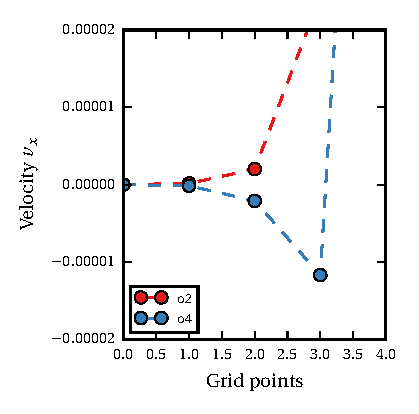
\includegraphics{gfx/immersed_boundary/poiseuille_flow/discussion/stencil.pdf}
            }}%
    \qquad
    \subfloat[label 2]{{
    \label{fig:example_b}%
      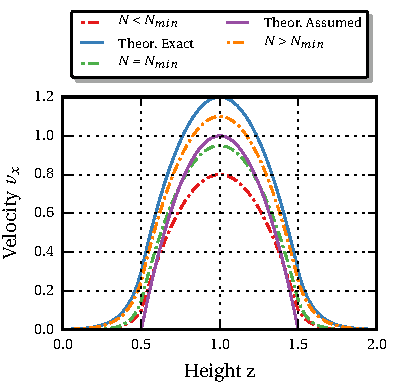
\includegraphics{gfx/immersed_boundary/poiseuille_flow/discussion/profile.pdf}
        }}%

\end{figure}

The grid convergency study with a constant Reynolds number and variable damping rate, generates an error
which increases simulatenous with the grid resolution.
An explanation for this behavior can by given by revising the theoretical solution
and the finite difference stencils at the immersed boundary.

The error for both method does not converge towards zero, which means there has to be some discrepancy to the theoretical solution given by
Eq. \ref{vali:pflow_theosol}.
For a constant $J$ there is an offset $C$ to the theoretical solution,
which is given by the equillibrium accord to Eq.  \ref{valid:steady_state_pflow}.
This means that the theoretical solution which was assumed in the first place, is wrong for the Volume-Penalization method.
An additional offset in the flow, which is dependent of the damping rate $J$ has to be considered.
For a low resolution, the profile of the 2nd order method is closer to the assumed theoretical, which results in a smaller
error. With an increase to a higher resolution the error with respect to the real solution decreases.

An explanation for the convergence of the 4th order can be given by furthermore considering the descrization error at the immersed boundaries.
Fig. \ref{fig:example_a} shows exemplary the velocity profile near to the immersed boundary, for the Volume-Penalization method of 2nd and 4th order
at a resolution of $N=100$.
It can be seen that the velocity profile for the 4th order method, is slighty negative.
The reason for this is the use of a 5-Point stencil for the discretization.
The stencil reaches over the immersed boundary which results in a wrong computation of the laplacian.
An explanation for the 4th order convergence is given by the velocity profiles for different resolutions,
as shown schematically in Fig. \label{fig:example_b}.
\footnote{The difference in the computed velocity profiles is barely visible, therefore an exaggerated version is used.}
The velocity profiles for three different resolutions are considered for a constant $J$,
the minimum of the error shall be defined as $N_{min}$.
Due to the negative velocity at the boundary the first profile $N<N_{min}$ lies below the theoretical assumed.
The second profile is at $N=N_{min}$. The error at the boundary is smaller due to the increase of the resolution.
The profile overlaps best with the theoretical solution resulting in the minimal error.
With a further increase of the resolution  $N>N_{min}$ the velocity profile drifts away from the theoretical solution,
the error increases.  Finally the method converges towards the same solution as the 2nd order scheme.


\subsubsection{Direct Forcing Method}

The results for the direct forcing method show that d


-We can see o4 not working reason is the same as we can se in Fig. n) , the laplacian is wrong caclulated at the point B.
As a results an error is induced at the boundaries of the domain.
The 2nd order scheme works perfectly as we compare it to the default implementation.

